\chapter{Demonstration Setup}
\label{sec:demo}
At the heart of our demonstration is a web-based ``top-$k$'' list
extraction user interface \cite{list-extractor}.

\begin{figure}[th]
	\centering
	\epsfig{file=./pics/Snapshot.eps,width=0.9\columnwidth}
\caption{The Top-K Extraction Web GUI: TryItOut}
\label{fig:gui}
\end{figure}

\begin{figure}[th]
	\centering
	\epsfig{file=./pics/benchmark1.eps,width=0.9\columnwidth}
\caption{The Top-K Extraction Web GUI: Benchmark}
\label{fig:gui2}
\end{figure}

\begin{figure}[th]
	\centering
	\epsfig{file=./pics/titleGUI2.eps,width=0.9\columnwidth}
\caption{The Top-K Extraction Web GUI: Title}
\label{fig:gui3}
\end{figure}

%Under Home tab, user can test any page by its URL, the system
%will retrieve the page in real time
%and attempt to extract a ``top-$k$'' list from it.
%The output includes the page title, running time, number $k$, concepts
%as well as the ``top-k list''.
%Under Benchmark tab, we provide a benchmark collection of 100 ``top-$k$'' pages.
%Under Title tab, user can type a string as input,
%and the system will analyze it as a page title and return detailed result.

In TryItOut section, you can type in the URL in the textbox and click "Extract" button, the system will retrieve the page in real time and attempt to extract a ��top-k�� list from it. The output result includes the page title, running time (in millisecond), number k, concepts as well as the ��top-k list��. Both the result and the original page will be presented after extraction.
A screenshot of the TryItOut Section with blow-ups of extracted content
is shown in Figure \ref{fig:gui}.


In Benchmark section, we list 100 "top-k" pages with their URLs. If you want to test anyone of them, you can click "Test Me" button, the web will redirect to TryItOut and show you the result. Also if you want to test the whole benchmark, you can click "Test All" (in the bottom), the system will process through the benchmark and send you a result file in XML format.
A screenshot of the Benchmark Section with blow-ups of test bottoms
is shown in Figure \ref{fig:gui2}.


We also provide Title section to test page title. In this section, you can type a string as input in the textbox, then click "Parse" button, and the system will analyze it as a page title and return detailed result.
A screenshot of the Title Section
is shown in Figure \ref{fig:gui3}.
